\section{Link-State Database}
\label{sec:lsdb}

The Link-State Database (LSDB) holds LSA information distributed by
other routers in the network.  The LSDB stores all types of LSAs and
will trigger events when a new LSA is added, updated, or expires.  The
LSDB also handles LSA retrieval, performs LSA builds, and triggers
routing table calculations.

\subsection{Retrieving an LSA}

The LSDB provides the \texttt{Lsdb::expressInterest()} method as a
public interface to retrieve an LSA from the network.  If LSA Data is
returned, the LSDB will validate the Data using the Validator
module. Then, it will perform the necessary LSDB modifications.  If
the LSA Interest times out, the LSDB will retry until it reaches a
configurable maximum number of tries, or a configurable deadline
passes.

The LSDB uses the SegmentFetcher system to retrieve LSAs. LSAs very
often will exceed the maximum NDN packet size. In these cases, the LSA
needs to be split into segments to be sent, so the LSDB uses the
SegmentFetcher to send all LSAs. The SegmentFetcher can decide if the
data actually needs to be split.

\subsection{General Procedure}

The LSDB is responsible for building, installing, and publishing
NLSR's LSAs, as well as for installing and processing LSAs from other
NSLRs. Generally, the functions of the LSDB are:
\begin{itemize}
\item Schedule the building of an LSA.
\item Building the LSA.
\item Installing the LSA into the LSDB.
\end{itemize}

\subsection{Scheduling LSA Builds}
LSAs need to be rebuilt whenever the routing information NLSR has
changes. This includes events like neighbors becoming active, or when
a prefix for advertisement is inserted by the Prefix Update Processor,
which would cause an adjacency LSA or a name LSA rebuild,
respectively. To improve performance, instead of directly building
adjacency LSAs the first request schedules the build, and build requests
that occur after the scheduling but before the actual event are
aggregated (in other words, ignored), because they will be satisfied
by the already-scheduled build. Some specifics are shown below.
below.
\begin{itemize}
\item \textbf{Adjacency LSAs} -- will only be scheduled if link-state
  routing is enabled. In particular, this means Adjacency LSA builds
  will \emph{not} occur if hyperbolic routing is enabled. Note that
  adjacency LSAs will be built if dry-run hyperbolic routing is
  enabled, as the network is still using link-state routing to
  calculate paths.
\end{itemize}

\subsection{Building LSAs}
Building LSAs has a part common to all LSAs and a part specific to
each LSA type. For example, all LSA types increment sequence number
and have the same expiration length, and of course come from the same
router. Additionally, all LSA builds cause a sync update
publishing. However, each type of LSA includes different data, to
represent different kinds of information that NLSR
has. (Section~\ref{sec:lsas}) In particular:
\begin{itemize}
  \item \textbf{Adjacency LSAs} -- the number and a list of active
    neighbors is included.
  \item \textbf{Coordinate LSAs} -- the hyperbolic radius and all
    hyperbolic angles are included.
  \item \textbf{Name LSAs} -- the list of name prefixes that are
    accessible at this router is included.
\end{itemize}

\subsection{Installing and Processing LSAs}
LSA installation procedure is mostly the same across any type of LSA,
but each type also has installation behavior specific to that type,
too. For any LSA type, we need to schedule an expiration event, and we
need to update several fields in the LSA. However, installing an
adjacency or coordinate LSA causes a Routing Table calculation, but a
name LSA does not, for example.
%%| Not yet true, but it should be true!
Additionally, the name of the origin router is added as a ``routable prefix'' in the NPT. (Section~\ref{sec:npt}).
\begin{itemize}
  \item \textbf{Adjacency LSAs} -- each adjacency in the LSA will be
    added as a ``routable prefix'' to the NPT. If the adjacencies have
    changed since the last version of this LSA, a Routing Table
    calculation needs to be scheduled, because the state of the
    network has changed. Of course, this is necessarily true if the
    LSA is new to us. Important to note is that we will also install
    and process \emph{our own} adjacency LSA in this way.
  \item \textbf{Coordinate LSAs} -- the router that the LSA is from
    will be added as a ``routable prefix'' to the NPT. If the radius
    and coordinates have changed since the last version of this LSA, a
    Routing Table calculation needs to be scheduled, because the state
    of the network has changed. As above, this is true for a new
    LSA. This is only done if the LSA is from a foreign router.
  \item \textbf{Name LSAs} -- each name prefix in the LSA will be
    added to our NPT. This is only done if the LSA is from a foreign
    router.
\end{itemize}

\subsection{LSA Expiration}
LSAs expire so that the network can clean up when a router
crashes. The amount of time an LSA lasts is configurable. When an LSA
expires, we refresh it if it's our LSA, and remove it from the LSDB if
not. There is a ``grace period'' window that is appended to the end of
the expiration period of all LSAs, to provide time for the originating
router to refresh the LSA and for it to propagate back to us. In all
expiration cases, the name of the origin router will be removed from
the NPT. What happens when an LSA is removed from the LSDB differs
based on the type of LSA:
\begin{itemize}
  \item \textbf{Adjacency LSAs} -- a Routing Table calculation needs to occur,
    since the state of the network has changed, at least from our
    perspective.
  \item \textbf{Coordinate LSAs} -- a Routing Table calculation needs to occur,
    since the state of the network has changed, at least from our
    perspective.
  \item \textbf{Name LSAs} -- the name prefixes in the LSA are removed from the
    NPT.
\end{itemize}

\subsection{LSA Refreshment}
NLSR will only refresh its own LSAs. Additionally, the procedure for refreshing an LSA is the same for all types:
\begin{itemize}
\item Increment the LSA sequence number
\item Schedule another expiration event. The length of time to wait
  until refreshing is configurable, but it should probably be lower
  than the expiration time that was set when building the LSA
  initially. This prevents other routers from deleting our LSAs
  because the network is slow, for instance. The length of time is set
  by \texttt{lsa-refresh-time} in the configuration file.
\item Publish an update to sync
\end{itemize}

\begin{figure}[h]
\center
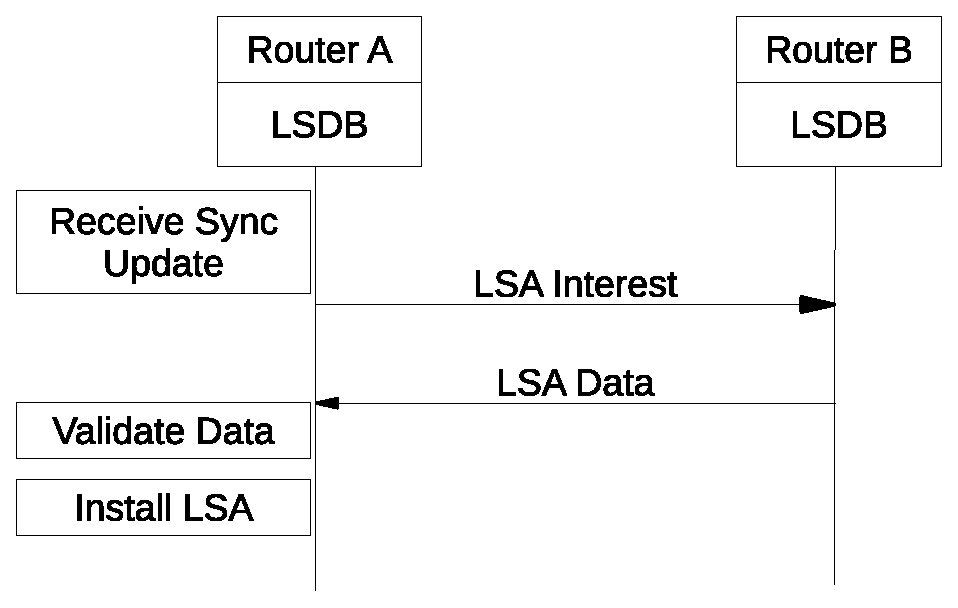
\includegraphics[width=0.5\linewidth]{figures/generic-lsdb-flow}
\label{fig:generic-lsdb-flow}
\caption{The general LSDB logic for each LSA type}
\end{figure}
